\subsubsection{Increasing number of destination nodes}
\label{sec:incrdestnodes}

\begin{figure*}%[!htbp]
        \centering
        \begin{subfigure}[b]{0.32\textwidth}
                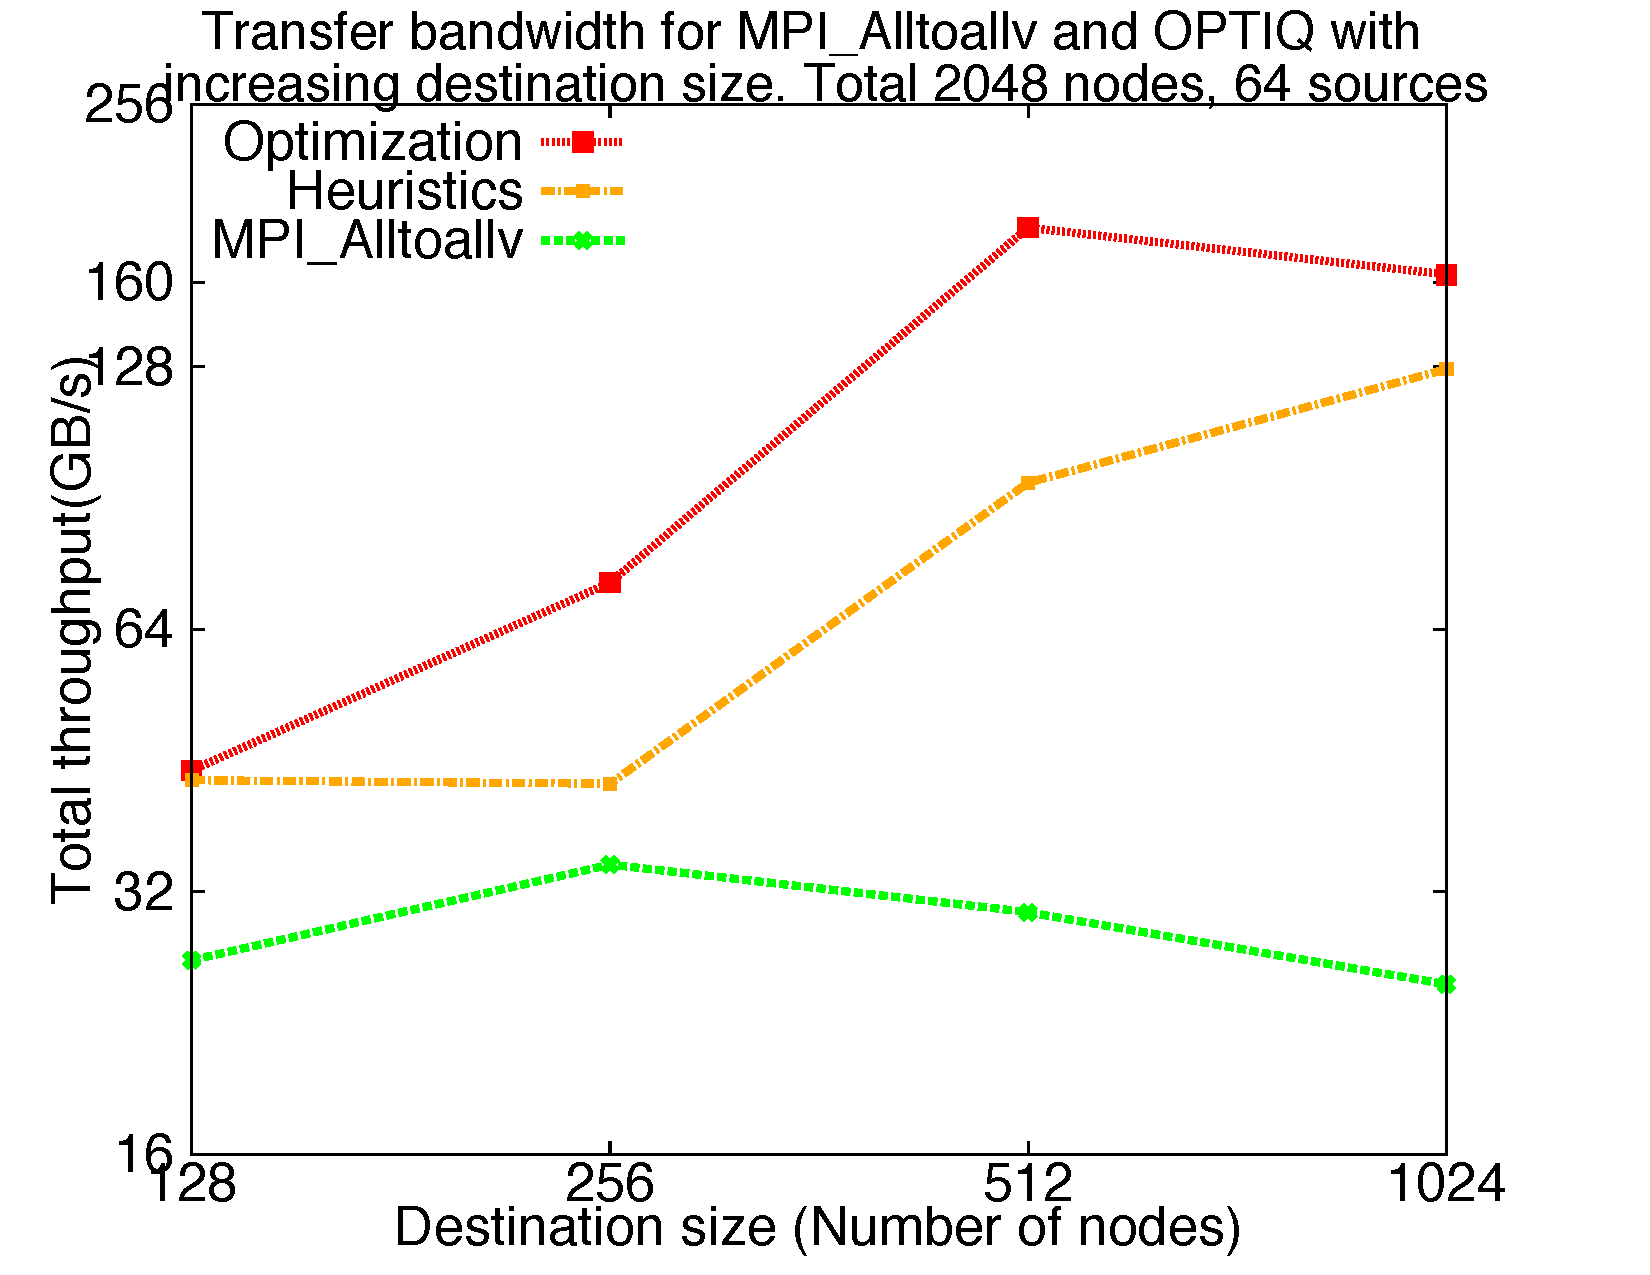
\includegraphics[width=\textwidth]{figures/incrsize_disjoint.pdf}
                \caption{Disjoint}
                \label{fig:incrsize_disjoint}
        \end{subfigure}%
        ~ %add desired spacing between images, e. g. ~, \quad, \qquad, \hfill etc.
          %(or a blank line to force the subfigure onto a new line)
        \begin{subfigure}[b]{0.32\textwidth}
                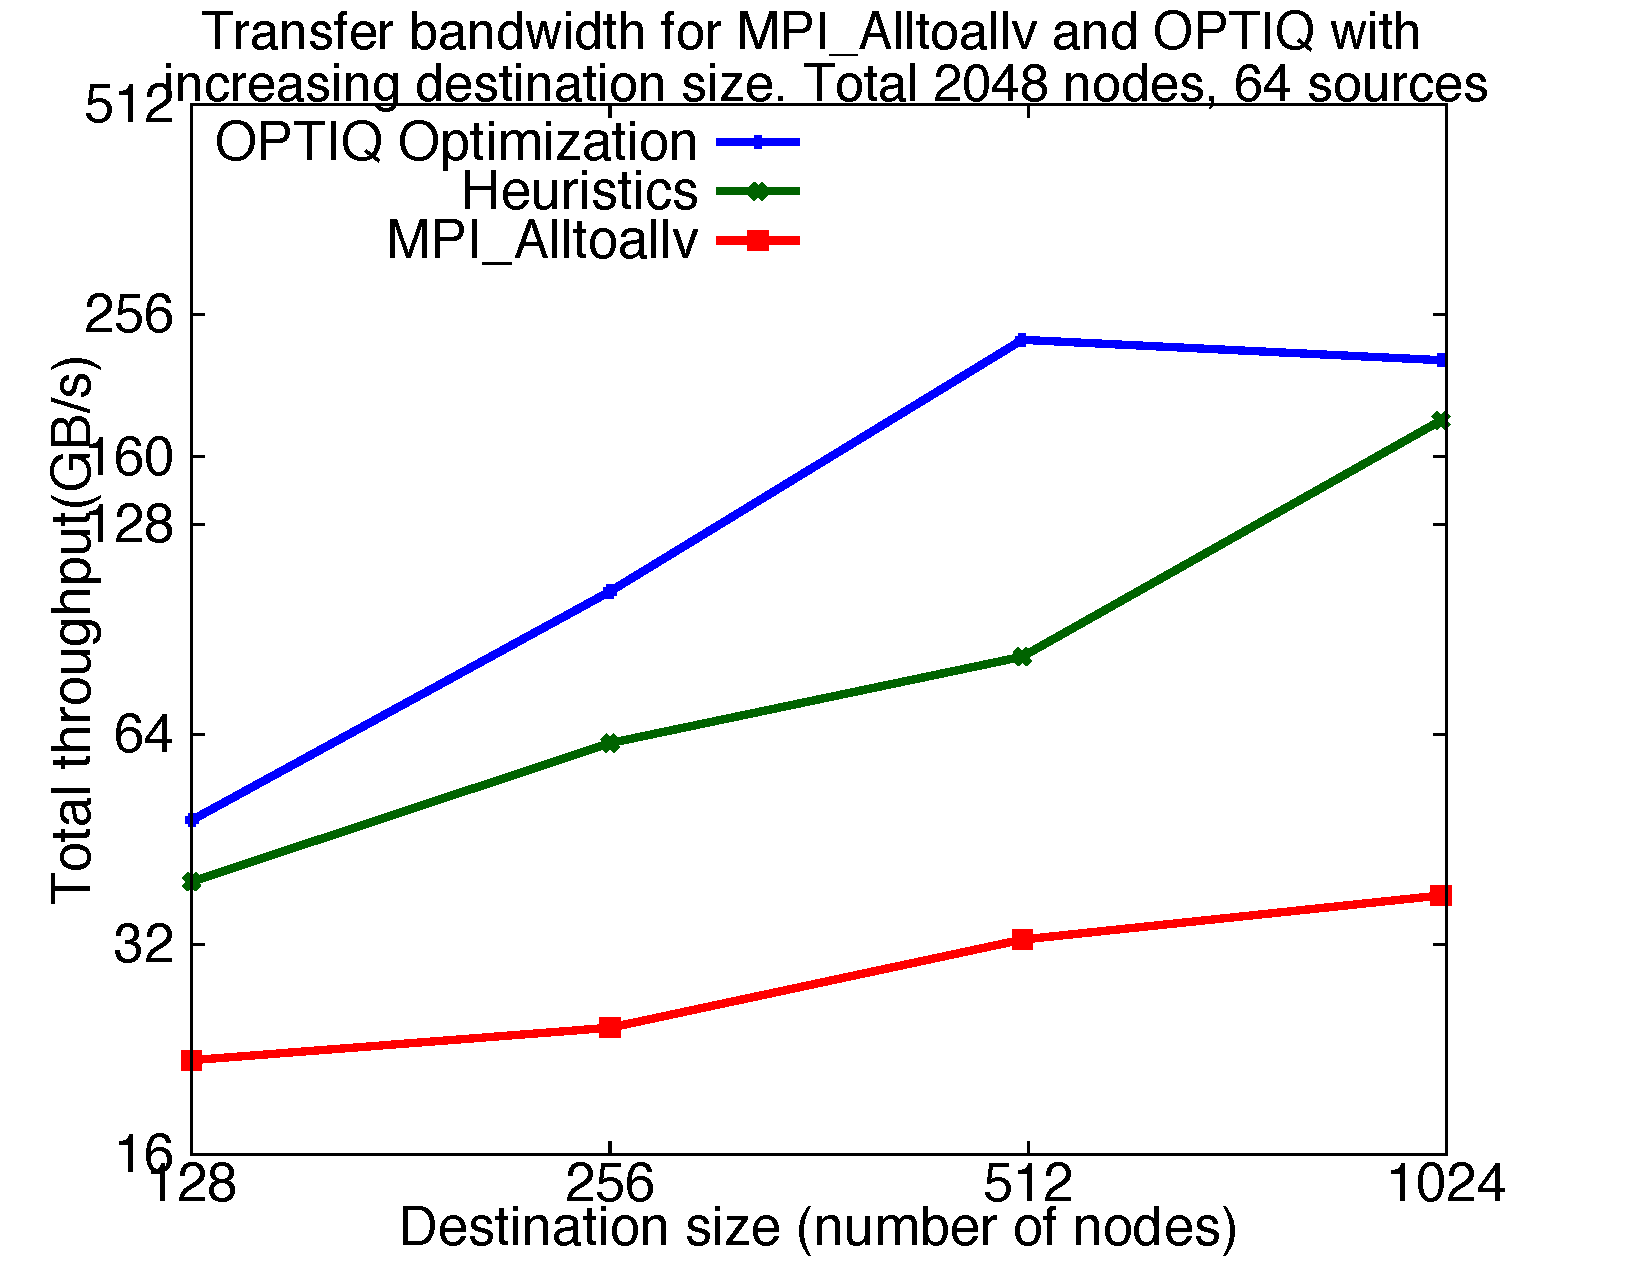
\includegraphics[width=\textwidth]{figures/incrsize_overlap}
                \caption{Overlap}
                \label{fig:incrsize_overlap}
        \end{subfigure}
        ~ %add desired spacing between images, e. g. ~, \quad, \qquad, \hfill etc.
          %(or a blank line to force the subfigure onto a new line)
        \begin{subfigure}[b]{0.32\textwidth}
                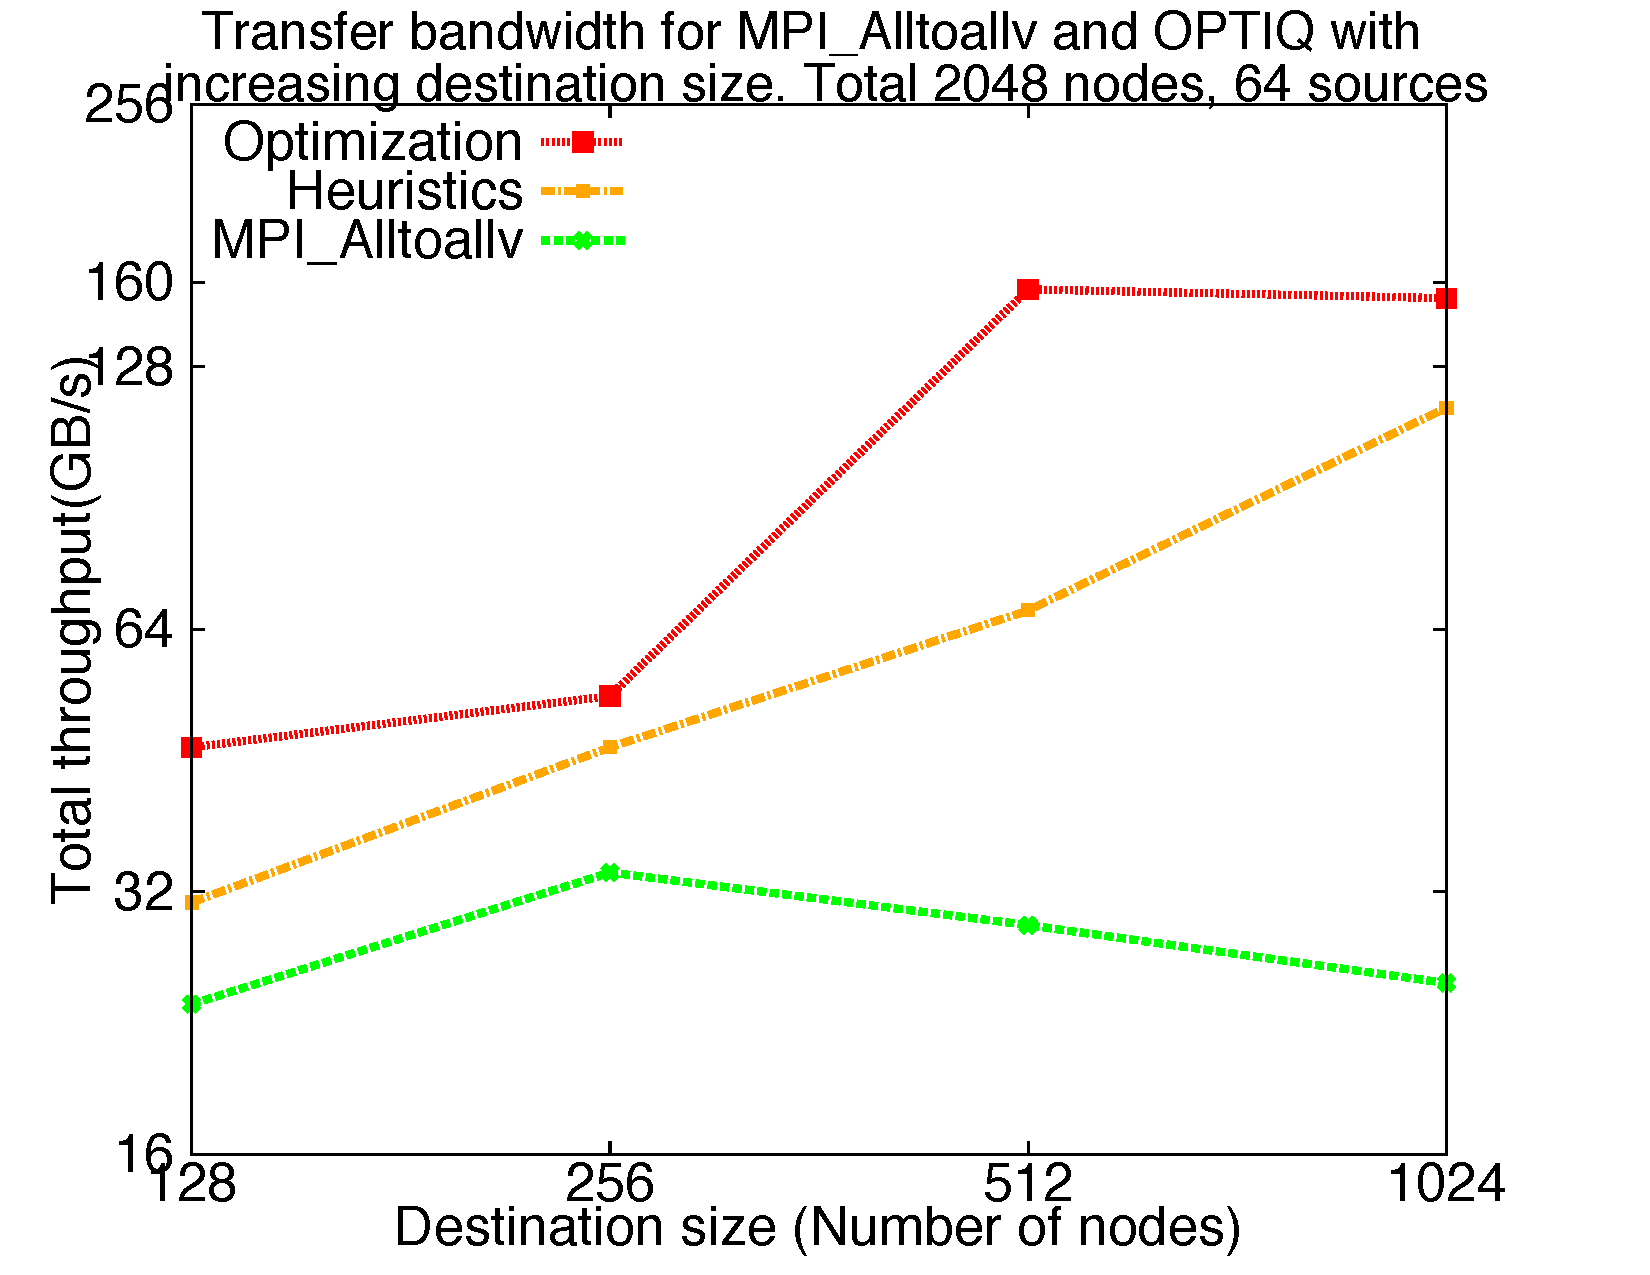
\includegraphics[width=\textwidth]{figures/incrsize_subset}
                \caption{Subset}
                \label{fig:incrsize_subset}
        \end{subfigure}
        \caption{Total data movement throughput with increasing number of destination nodes.}
        \label{fig:incrsize}
\end{figure*}

In this experiment we use a partition of 2048 nodes. We keep the number of source nodes constant (64 nodes) and increase the number of destination nodes from 128 to 256, 512 and 1024 nodes. Each source node communicates with k destination nodes where k = 2, 4, 8 and 16 respectively. Node $x$ communicates with nodes $k\cdot x$, $k\cdot x+1$, ..., $k\cdot x+(k-1)$. There is 1 MPI/PAMI rank per node. Each pair of communication involves 8 MB of data transfer. The performance of OPT, HEU and MPI for disjoint, overlap and subset patterns is shown in Figure \ref{fig:incrsize}. With increase in number of destination nodes, OPT and HEU yields better performance than MPI\_Alltoallv. The throughput of OPT increases for destination sizes of 256 and 512 but slightly reduces at 1024 nodes, whereas the throughput of HEU increases as the destination size increases. This is because OPT tries to globally balance load while distributing data among all paths, whereas HEU ensures load limit per path but distributes data for each communication pair, oblivious of the global load. With higher number of destination nodes, the number of paths with overlapping links increases. Another reason for OPT's drop in performance is because we do not consider the underlying synchronization overheads in the data transfer optimization formulation.  
%TODO why is this the case? higher load for OPT for 1024? review the above reason, does it seem correct?
%As Figure \ref{fig:incrsize} shows, as we increase the ratio between the sources and destinations by increasing the destination sizes, both Optimization and Heuristics have better performance than MPI\_Alltoallv. In addition, they work better at scale than MPI\_Alltoallv. The throughput of Optimization approach increases for destination sizes of 256 and 512 but slightly reduces at 1024 nodes, while the throughput of Heuristic approach increases as the destination size increases.
%\begin{table*}%[!htbp]
%   \centering
%    \begin{tabular}{| l | p{0.5cm} | p{0.5cm} | p{0.6cm} | p{0.6cm} | p{0.5cm} | p{0.5cm} |p{0.6cm} | p{0.6cm} | p{0.5cm} | p{0.5cm} |p{0.6cm} | p{0.6cm} |p{0.5cm} | p{0.5cm} |p{0.6cm} | p{0.6cm} |}
%    \hline
%     \#destinations & \multicolumn{4}{ c | }{128} & \multicolumn{4}{ c| }{256} & \multicolumn{4}{ c| }{512} & \multicolumn{4}{ c| }{1024} \\ \hline
%     Patterns & {Max} & Avg & OPT \#Paths & HEU \#Paths & Max & Avg & OPT \#Paths & HEU \#Paths & Max & Avg & OPT \#Paths & HEU \#Paths & Max & Avg & OPT \#Paths & HEU \#Paths \\ \hline
%     Disjoint & 15 & 9.50 & 355 & 1021 & 18 & 10.44 & 923 & 1386 & 20 & 10.44 & 1101 & 1978 & 21 & 10.19 & 1631 & 1958 \\ \hline
%     Overlap  & 11 & 6.25 & 476 & 2108 & 16 & 7.19 & 937 & 2864 & 18 & 8.38 & 1690 & 4064 & 21 & 9.12 & 2081 & 4710 \\ \hline
%     Subset   & 11 & 5.5  & 491 & 1799 & 16 & 6.69 & 665 & 2184 & 20 & 8.31 & 1255 & 3021 & 21 & 8.56 & 1551 & 3436\\ \hline
%    \end{tabular}
%    \caption{Maximum (Max) and average (Avg) distance (number of hops) and number of paths (Paths) between sources and destinations for different configurations on 2048 Mira nodes.}
%    \label{table:incrsize}
%\end{table*}
%TODO: what do you want to show through this table? number of paths for OPT increases but perf drops!
%instead, may be you can find the load information, and try to find the reason for OPT perf drop
%Table \ref{table:incrsize} shows  
